\section{Zielsetzung}

    \noindent In diesem Versuch soll die Dichte, Rauigkeit und Schichtdicke eines dünne Polystyrolfilms mit Hilfe der Röntgenreflektrometrie 
    ermittelt werden. 

\section{Theorie}

    \noindent
    Die Probe wird mit Röntgenstrahlen, welche Wellenlängen zwischen $\lambda = \SI{0.1}{\angstrom}$ und $\lambda = \SI{10}{\angstrom}$ haben, 
    untersucht. 

    \subsection{Brechung}

        \noindent
        Trifft eine elektromagnetische Welle auf eine Grenzfläche zweier Medien, die verschieden Brechungsindizes $n_1 \neq n_2$ haben, findet Brechung
        statt. Nach dem Snelliusschen Brechungsgesetz 
        \begin{equation*}
            \frac{n_1}{n_2} = \frac{\cos(\alpha_2)}{\cos(\alpha_1)}
        \end{equation*}
        ändert sich die Ausbreitungsrichtung der Welle. 
        Der Brechungsindex kann über 
        \begin{equation*}
            n = 1 - \delta + \symup{i} \beta 
        \end{equation*}
        ausgedrückt werden, wobei $\delta$ ein Korrekturterm der Größenordnung $\num{10e-6}$ ist und $\beta$ für die Absorbtion der Strahlung in dem 
        bestimmten Medium steht. 
        Für Röntgenstrahlung ist $\delta > 0$, der Realteil des Brechungsindex dementsprechend kleiner als eins. 
        Dies ermöglicht die äußere Totalreflektion, die nur beim Übergang eines optischen dichteren Mediums in ein optisch dünneres Medium auftreten kann, 
        solange die Grenzfläche zwischen der Medien eine homogene Ebene bildet. 
        Der kritische Winkel $\alpha_\text{c}$, bei dem es zur Totalreflexion kommt, kann bei Vernachlässigung der Absorption und für kleine Winkel als 
        \begin{equation*}
            \sqrt{2 \delta} \approx \alpha_\text{c} = \lambda \sqrt{\frac{r_\text{e} \rho}{\pi}}
        \end{equation*}
        ausgedrückt werden, wobei $r_\text{e}$ der klassische Elektronenradius ist und $\rho$ die Elektronendichte des Materials. 

    \subsection{Fresnel Formel}

        \noindent 
        Die Intensitäten der reflektierten und transmittierten Anteile von elektromagnetischen Wellen können durch die Fresnel Formel beschrieben werden. 
        Hier wird keine Unterscheidung zwischen $s-$ und $p-$ Polarisation gemacht, da diese bei sehr ähnlichen Brechungsindizes $n_1 \approx n_2$ 
        nicht notwendig ist. 
        Es ergeben sich 
        \begin{align*}
            r &= \frac{n \cos(\alpha_1) - n \cos(\alpha_2)}{n \cos(\alpha_1) + n \cos(\alpha_2)} \\
            t &= \frac{2 n \cos(\alpha_1)}{n \cos(\alpha_1) + n \cos(\alpha_2)}\, .
        \end{align*}

        \noindent
        % Die Fresnelreflektivität ist näherungsweise für Röntgenstrahlung und $\alpha_i > 3 \alpha_\text{c}$ 
        % \begin{equation*}
        %     R_f = \biggl(\frac{\alpha_\text{c}}{2 \alpha_i}\biggr)\, .
        % \end{equation*}

    \subsection{Mehrschichtsystem}

        \noindent 
        Besteht die Probe nicht nur aus einem Material, sondern aus mehreren Schichten, so wird an jeder Grenzfläche ein Teil der Strahlung reflektiert und 
        der andere Teil gebrochen und transmittiert. Unter den an verschiedenen Grenzflächen reflektierten Anteilen tritt Interferenz auf. In 
        \autoref{fig:bsp_kiessig} ist die Reflektivität abhängig vom Einfallswinkel aufgetragen, es handelt sich dort um ein Material mit zwei Schichten. 
        \begin{figure}
            \centering
            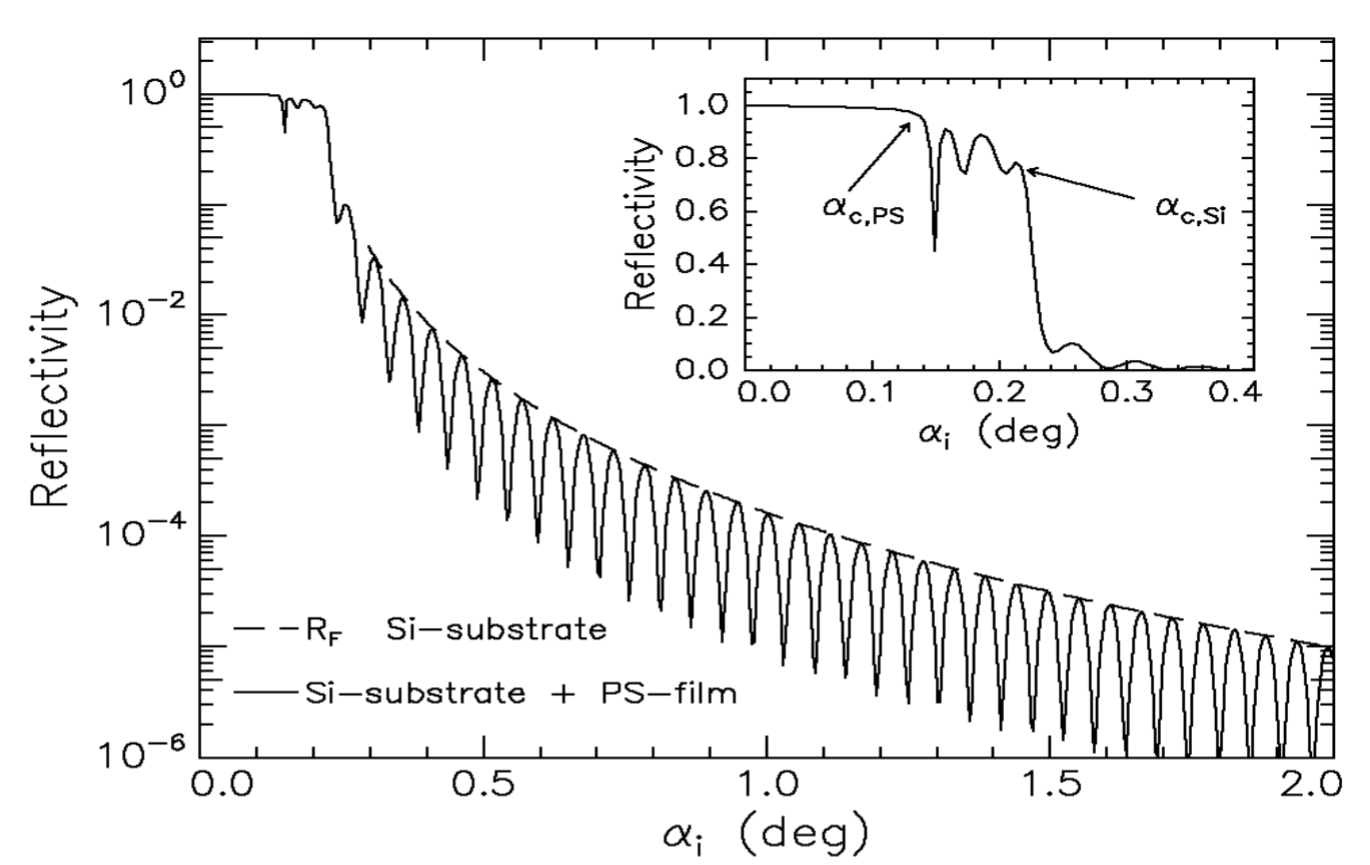
\includegraphics[width=\textwidth]{latex/images/reflectivity.png}
            \caption{Die Reflektivität eines Siliziumwafers mit einer $\SI{800}{\angstrom}$ dicken Polystyrolschicht aufgetragen gegen den Einfallswinkel der Röntgenstrahlung}
            \label{fig:bsp_kiessig}
        \end{figure}
        In dem vergrößerten Bereich sind zwei Winkel $\alpha_\text{c}$ aufgetragen, welche für die Totalreflexion der Röntgenstrahlung an der Polystyrolschicht 
        und an dem Siliziumwafer stehen. Anschließend zeigt die Reflektivität einen Abfall auf. Dabei werden die sogenannten Kiessig-Oszillationen 
        sichtbar. Aus dem Abstand aufeinanderfolgender Minima (oder Maxima) kann die Dicke der obersten Schicht ermittelt werden, da der Gangunterschied 
        der interferierenden Wellen für destruktive Interferenz ein Vielfaches von $\frac{\pi}{2}$ sein muss. 
        Es folgt
        \begin{equation*}
            d = \frac{2 \pi}{\delta q_z} = \frac{\lambda}{2 \delta \alpha_1}\, ,
        \end{equation*} 
        wobei $\vec{q} = \vec{k_2} - \vec{k_1}$ und $q_z = 2 k \sin(\alpha_1)$ gilt.

         
        \begin{figure}%
            \centering%
            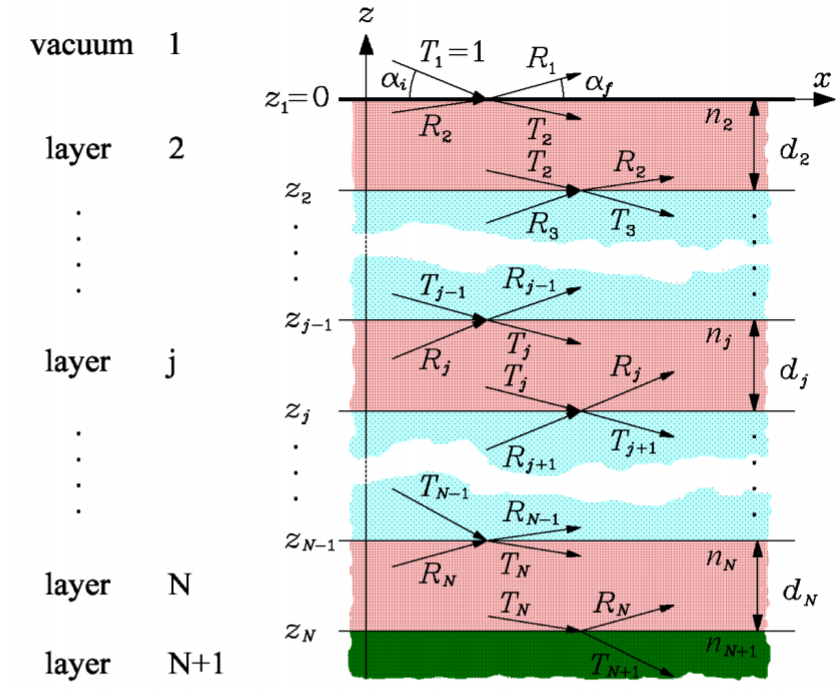
\includegraphics[width=0.5\textwidth]{latex/images/layers.png}%
            \caption{Schematische Darstellung eines Mehrschichtensystems mit $N+1$ Schichten.}%
            \label{fig:layers}%
        \end{figure}
        \noindent
        Bei einem System mit mehr Schichten, wie es in \autoref{fig:layers} zu sehen ist, kann die Reflektivität mithilfe des rekursiven Parratt-Algorithmus 
        berechnet werden. Hier wird angenommen, dass die unterste Schicht unendlich dick ist und hier keine Reflexion stattfindet. Es gilt also 
        $R_{N+1} = 0 = X_{N+1}$, dies dient als Startpunkt der Rekursion. Der Parratt-Algorithmus sieht folgendermaßen aus
        \begin{equation*}
            X_j = \frac{R_j}{T_j} = \exp\biggl( - 2 \symup{i} k_{z,j}z_j\biggr) \cdot \frac{r_{j, j+1} + X_{j+1}\exp\biggl(2 \symup{i} k_{z, j+1} z_j\biggr)}{1+ r_{j, j+1} X_{j+1}\exp\biggl(2 \symup{i} k_{z, j+1} z_j\biggr)}\, ,
        \end{equation*}
        hierbei steht $r_{j, j+1}$ für die Fresnelreflektivität der $j$-ten Grenzfläche und $k_{z,j}$ für die $z$-Komponente des Wellenvektors in der $j$-ten Schicht. 

        \noindent
        Um die Rauigkeit der Grenzflächer einzubeziehen, wird die \enquote{root-mean-square}-Rauigkeit eingeführt
        \begin{equation*}
            \sigma_j^2 = \int (z - z_j)^2 P_j(z)\, \symup{d}z\, .
        \end{equation*}
        Es steht $z_j$ für die Position der $j$-ten Grenzfläche und $P_j(z)$ für die Wahrscheinlichkeit, dass sich die Grenzschicht im Intervall 
        $ z + z_j, z + z_j + $. 
        Der Parratt-Algorithmus arbeitet dann mit den modifizierten Fresnel-Koeffizienten
        \begin{align*}
            \tilde{r}_{j, j+1} &= r_{j, j+1} \cdot \exp\biggl( - 2 k_{z, j} k_{z, j+1} \sigma_j^2\biggr) \\
            \tilde{t}_{j, j+1} &= t_{j, j+1} \cdot \exp\biggl( (k_{z,j} - k_{z, j+1})^2 \frac{\sigma_j^2}{2}\biggr)\, .
        \end{align*}

    \subsection{Geometriefaktor und Geometriewinkel}

        \noindent 
        In \autoref{fig:gfaktor} ist veranschaulicht, dass erst ab einem genügend großen Einfallswinkel der gesamte Strahl die Oberfläche trifft. 
        Dieser Winkel wird Geometriewinkel $\alpha_\text{g}$ genannt. 
        \begin{figure}
            \centering
            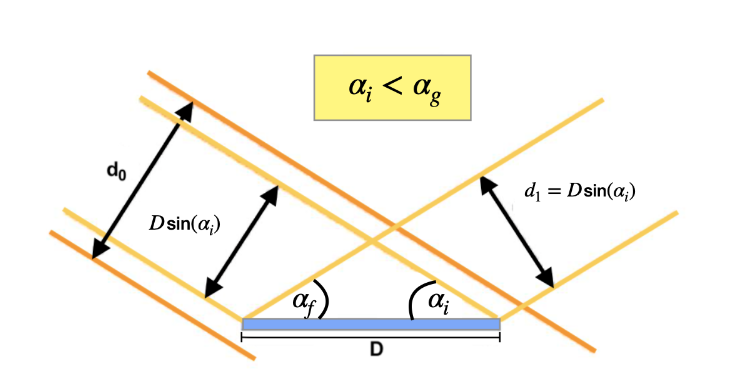
\includegraphics[width=0.7\textwidth]{latex/images/gfaktor.png}
            \caption{Strahlverlauf zur Veranschaulichung des Geometriewinekls $G$. \cite{V44}}
            \label{fig:gfaktor}
        \end{figure}
        Der Geometriefaktor wird für eine Probe des Durchmessers $D$ und bei einer 
        Strahlhöhe von $d_0$ geschrieben als 
        \begin{equation*}
            G = \begin{cases}
                \frac{D \sin{\alpha_i}}{d_0} & \alpha_i < \alpha_\text{g} \\
                1 & \alpha_i > \alpha_\text{g}
            \end{cases}\, .
        \end{equation*}
        Er berücksichtigt die Tatsache, dass kleine Winkel unterrepräsentiert sind, und durch ihn können die Daten später skaliert werden. 